\documentclass[]{IEEEtran}
% Your packages go here
\usepackage[utf8]{inputenc}
\usepackage{graphicx}
\usepackage{grffile}
\usepackage{gensymb}
\usepackage{amsmath}
\usepackage{amssymb}
\usepackage{listings}
\usepackage{mathtools}
\usepackage{subfig}
\usepackage{xcolor}
\usepackage{multirow}
\usepackage{xfrac}
\usepackage{amsmath}
\usepackage{float}
\DeclareMathOperator{\atantwo}{atan2}

\DeclareMathOperator{\arctantwo}{arctan2}


\definecolor{codegreen}{rgb}{0,0.6,0}
\definecolor{codegray}{rgb}{0.5,0.5,0.5}
\definecolor{codepurple}{rgb}{0.58,0,0.82}
\definecolor{backcolour}{rgb}{0.95,0.95,0.92}

\lstdefinestyle{mystyle}{
    backgroundcolor=\color{backcolour},   
    commentstyle=\color{codegreen},
    keywordstyle=\color{magenta},
    numberstyle=\tiny\color{codegray},
    stringstyle=\color{codepurple},
    basicstyle=\ttfamily\footnotesize,
    breakatwhitespace=false,         
    breaklines=true,                 
    captionpos=b,                    
    keepspaces=true,                 
    numbers=left,                    
    numbersep=5pt,                  
    showspaces=false,                
    showstringspaces=false,
    showtabs=false,                  
    tabsize=2
}
 
\lstset{style=mystyle}
 
\usepackage{lipsum}% http://ctan.org/pkg/lipsum
\usepackage{graphicx}% http://ctan.org/pkg/graphicx

\def\footnoterule{\relax%
  \kern-2pt
  \hbox to \columnwidth{\hfill\vrule width 0.7\columnwidth height 0.4pt\hfill}
  \kern4.6pt}
\makeatother

\renewcommand{\lstlistingname}{Algorithm}% Listing -> Algorithm
\usepackage[noadjust]{cite}
\markboth{MO433 - Unsupervised Machine Learning }{}

% \usepackage{graphicx}
% \graphicspath{{../output/}}

\begin{document}

\title{Final Project}
\author{Ivan Lima do Espirito Santo \thanks{RA: 956694 - i956694@g.unicamp.br}\\ Rosa Yuliana Gabriela Paccotacya Yanque \thanks{RA: 263068 - r263068@dac.unicamp.br} \\ Thiago Gomes Marçal Pereira \thanks{RA: 189691 - t189691@g.unicamp.br}}

\maketitle
%%\begin{abstract}
%%\end{abstract}

\section{Goal}
Image-to-Image translation refers to an area of Unsupervised Machine Learning, that aims to taking images from one domain and transforming them so that they have styles (or characteristics) of images from another domain.\\\\
Images can be easily related to each other, like Satellite Images to Map Images, and the problem could be solved by a Deep Neural Network, with simple input/output pairs. But, it can also be really hard to map images to each other, like paintings and real locations. And also images that might be almost impossible to map, like Horses to Zebras, as finding situations in which pairs of images where they would be in the same position and location would be extremely hard. \\\\
Our proposal is to follow the later, with solutions that base on GAN networks, in a way that it's able to learn not only the style, but characteristics of the image elements (Horse or zebra), and translate them to the other image, even if they are not directly mapped. In some approaches, this is also reversible.
Unpaired Image-to-Image Translation using Cycle-Consistent Adversarial Networks


\section{Image to Image Translation}\label{}
Consider a problem of creating a image. For instance, we could draw a rough representation of an object and try to create a more accurate image from this rough representation. For this approach to be attainable, we need first a dataset with a certain amount of these rough images in pairs with their accurate images. Once these pairs of images are available for a lot of different objects (or people, animals, landscape, etc) the problem of creating a new image from a new rough representation is a matter of learning the translation function. However, this approach relies on data labeling, which is expensive and not desirable. On the other hand, consider the problem of creating images, but this time you do not have pairs of them to train the translation function. All you have is different images, with different styles. Satellite images and google map drawings, horses and zebras, landscape photos, and landscape paintings are all similar in some sense. We can posit they differ in style. Therefore, we can think of image translation as an attempt to creating a new image by applying the style of other images. For instance, we can translate a photo image of a landscape into a famous painting style. Because the images do not need to be available in pairs, this approach is known as unpaired. One way to achieve unpaired image-to-image translation is through  Generative Adversarial Networks, which we discuss briefly in the section \ref{GANs}. In summary, the trick is learning to translate an image from $X$ to $Y$ by mapping $G : X$ to $Y$ in a way the distribution of images from $G(X)$ is as close as possible to the distribution $Y$. Moreover, the inverse mapping $F : Y$ to $X$ is possible and achieved as well (see section CGAN). 


\section{Generative Adversarial Networks}\label{GANs}
\subsection{GANs' concept  }
GANs' creates a generative models via an adversarial process, that simultaneously trains two models: a generative model $G$ that captures the data distribution and therefore generates samples, and a discriminative model $D$ that estimates the probability that a sample came from the training data rather than generated by $G$. In other words, the discriminative model tries to predict if the samples is real (from the training data) or fake (generated by the generative model), while the generative model tries to fool the the discriminative model generating samples as similar as possible to real ones. This setup is equivalent to a minimax two-players game. The training rule for $G$ is to maximize the probability of $D$ making a mistake. The samples generated in this way end up very similar to real samples as one can see the left face (real) and the generated face in figure~\ref{fig02}. ~\cite{Goodfellow2014GenerativeAN}.\par

\begin{figure}[ht]
  \centering
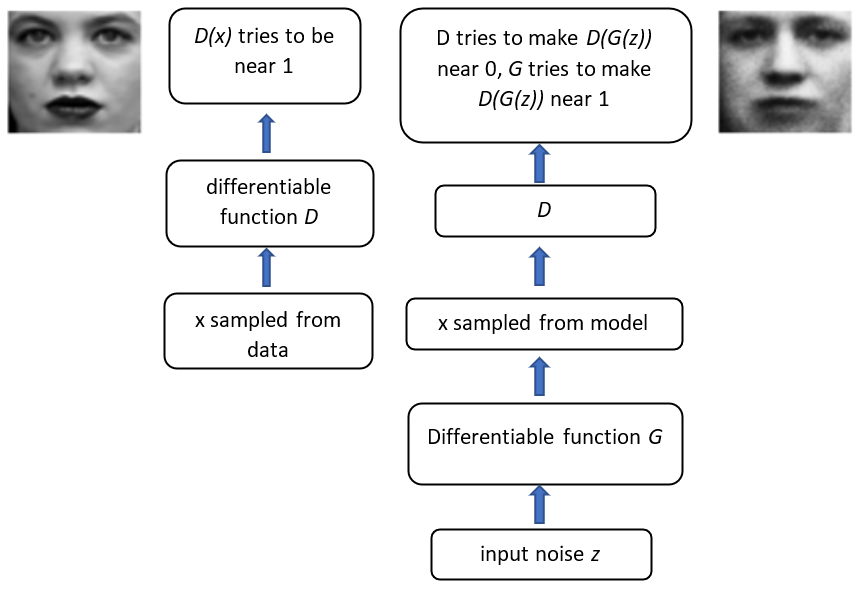
\includegraphics[width=0.5\textwidth]{./images/fig02_flux.png}
  \hspace{1mm}
  \caption{Figure from NeurIPS 2016 GAN Tutorial (Goodfellow)}
  \label{fig02}
\end{figure}

\subsection{GANs' Math}
We can mathematically describe the adversarial relationship between the generative model and the discriminative model with an equation of format~\ref{eq1}.

\begin{equation}
\begin{split}
\min _{G} \max _{D} V(D, G)=\\
\mathbb{E}_{x \sim p_{\text {data }}(x)}[\log D(x)]+\mathbb{E}_{z \sim p_{x}(z)}[\log (1-D(G(z)))]
\label{eq1}
\end{split}
\end{equation}

$G(z)$ generates $x$ images. Meanwhile the discriminator tries to classify (discriminate) which of $x$ are real versus generated. $\mathbb{E}_{x \sim p_{\text {data }}}$ is the real data distribution. The framework is such as it tries maximize the log probability under the discriminator which can have $0$ or $1$ sigmoid output. Discriminate will try to drive the output to 1 if it is real. Simultaneously, $\mathbb{E}_{z \sim p_{x}(z)}$ does the opposite. It tries to drive the discriminator to $0$ because it is not real. In other words, the discriminator is trying to assign $1$ to real and $0$ to fakes as accurate as possible. If we reach the Nash Equilibrium of this game, none of them can improve anymore, the generator should generate things that looks real. The discriminator at that point outputs $50/50$.
The game is defined to try to generate things as realistic as possible. The GANs algorithm presented in~\cite{Goodfellow2014GenerativeAN} is as follows: 

\begin{figure}[h]
\centering
\includegraphics[width=0.5\textwidth]{./images/pseudo.png}
\hspace{1mm}
\label{code}
\end{figure}


\subsection{The Optimal Discriminator}
 From equation~\ref{eq1}, using the integrals and changing the variable to write both integrals with respect to $x$ we have the following expressions:

\begin{equation}
\begin{split}
V(G, D) =\mathbb{E}_{x \sim p_{\text {data }}}[\log D(x)]+\mathbb{E}_{z \sim p(z)}[\log (1-D(G(z)))] \\
=\int_{x} p_{\text {data }}(x) \log D(x) d x+\int_{z} p(z) \log (1-D(G(z))) dz \\
=\int_{x} p_{\text {data }}(x) \log D(x) d x+\int_{x} p_{g}(x) \log (1-D(x)) dx \\
=\int_{x}\left[p_{\text {data }}(x) \log D(x)+p_{g}(x) \log (1-D(x))\right] dx
\end{split}
\end{equation}

By calculation the derivative with respect to $D(x)$ and set it equal to zero we have:
\begin{equation}
\begin{split}
\nabla_{y}[a \log y+b \log (1-y)]=0 \\
\Longrightarrow y^{*}=\frac{a}{a+b} \quad \forall \quad[a, b] \in \mathbb{R}^{2} \backslash[0,0]
\end{split}
\end{equation}

Therefore, the optimal discriminator will take the form of equation~\ref{opt}.

\begin{equation}
D^{*}(x)=\frac{p_{\text {data }}(x)}{\left(p_{\text {data }}(x)+p_{g}(x)\right)}
\label{opt}
\end{equation}

Inserting equation~\ref{opt} in the original objective expression~\ref{eq1}, we have expression~\ref{eq2}:

\begin{equation}
\begin{aligned}
V\left(G, D^{*}\right) =\mathbb{E}_{x \sim p_{\text {data }}}\left[\log D^{*}(x)\right]+\mathbb{E}_{x \sim p_{g}}\left[\log \left(1-D^{*}(x)\right)\right] \\
=\mathbb{E}_{x \sim p_{\text {data }}}\left[\log \frac{p_{\text {data }}(x)}{p_{\text {data }}(x)+p_{g}(x)}\right]+\mathbb{E}_{x \sim p_{g}}\left[\log \frac{p_{g}(x)}{p_{\text {data }}(x)+p_{g}(x)}\right] \\
=-\log (4)+K L\left(p_{\text {data }} \|\left(\frac{p_{\text {data }}+p_{g}}{2}\right)\right)+K L\left(p_{\mathrm{g}} \|\left(\frac{p_{\text {data }}+p_{g}}{2}\right)\right)
\end{aligned}
\label{eq2}
\end{equation}

where the KL terms are the Jensen-Shannon Divergence (JSD) of $p_{\text {data }}$ and $p_{g}$, which is  $\ge 0$. Notice that $V\left(G^{*}, D^{*}\right)=-\log (4) \text { when } p_{g}=p_{\text {data }}$.

\section{Unpaired Image-to-Image Translation}
Based on is explained before, GAN approach appears to be suitable to learn to translate between different domains without images pairs. When we have two sets of images $X$ and images $Y$, with GAN we may find a mapping $G$ that maps $X$ to $Y$ as close as they end up indistinguishable. However, this translation is not sufficient to guarantee that an individual $x$ and a output $y$ are a meaningful pair once there are many possible $G$. Furthermore, another practical problem is common during the optimization of the adversarial objective when all the images maps to the same output images due to mode collapse.\\
These problems claim for some improvements in the GAN approach to make it indeed suitable for the task of unpaired image-to-image translation. Aiming to address these issues, ~\cite{CycleGAN} implemented the concept of cycle consistency. When a translation $G$ maps the images from $X$ to images $Y$, also a translation $F$ maps them backwards, i.e. from $Y$ to $X$. In other words, instead of seeking any translation $G$, we seek for one that has an inverse $F$. The existence of $F$ is assumed, therefore both $G$ and $F$ are training simultaneously. The cycle consistency loss is then defined to make $F(G(x)) \approx x$  and $G(F(y)) \approx y$. Accordingly, for the unpaired image-to-image translation we have the final objective by combining one adversarial loss for $G$, one adversarial loss for $F$ and the cycle consistency loss. \\


\section{Formulation}
Given two domains $X$ (images of horses, for instance) and $Y$ (images of zebras, for instance), our aim is to learn a mapping function $G$ that maps $X$ to $Y$ and learn a mapping function $F$ that maps $Y$ to $X$. For each of them, we use two adversarial discriminators, $Dx$ and $Dy$. While $Dx$ aims to discriminate between images $x$ and translated images $F(y)$, $D(x)$ aims to discriminate between images $y$ and $G(x)$. See figure~\ref{2GANs}. 

\begin{figure}[ht]
  \centering
  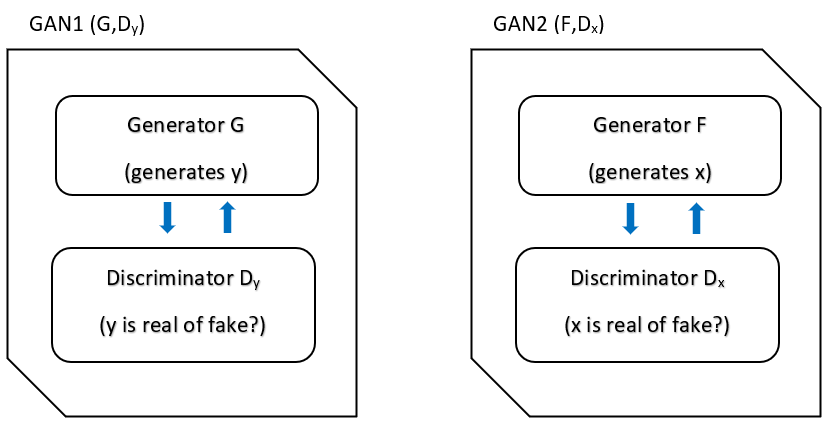
\includegraphics[width=0.4\textwidth]{./images/2GANs.png}
  \hspace{1mm}
   \caption{Two GANs formulation scheme.}
\label{2GANs}
\end{figure}\par

Besides the two adversarial loss for each of them, which push the generated images towards the target images, we need the cycle consistency loss to make $G$ and $F$ consistent with each other (avoid contradiction).\par 
Adversarial loss is core idea behind GANs. If we take the equation~\ref{eq1} and write it for the map $G:$ $X$ to $Y$, and the discriminator ${D}_{y}$ as shown in left side of figure~\ref{2GANs}, we have expressions~\ref{2GANs1}

\begin{equation}
\begin{split}
{ min }_{ G }{ max }_{ { D }_{ y } }\ell _{ GAN }(G,{ D }_{ y },X,Y)={ E }_{ y\sim p_{ { data } }(y) }[\log { D } _{ y }(y)]\\
+{ E }_{ x\sim p_{ data }(x) }[\log  (1-{ D }_{ y }(G(x))]
\label{2GANs1}
\end{split}
\end{equation}

$G$ tries to generate images similar to $Y$ while ${D}_{y}$ tries to recognize if they are real or fake. Real images come from $y$ and fake images are generated by $G(x)$. At the same time $G$ tries to minimize, ${D}_{y}$ tries to maximize.\par 

The same happens in the right side of the figure~\ref{2GANs}, but now for the map $F:$ $Y$ to $X$, as shown in the expression~\ref{2GANs2}

\begin{equation}
\begin{split}
{ min }_{ F }{ max }_{ { D }_{ x } }\ell _{ GAN }(F,{ D }_{ x },Y,X)={ E }_{ x\sim p_{ { data } }(x) }[\log { D } _{ x }(x)]\\
+{ E }_{ y\sim p_{ data }(y) }[\log  (1-{ D }_{ x }(F(y))]
\label{2GANs2}
\end{split}
\end{equation}

Each of these two adversarial losses represents the minmax game between the generator and the discriminator. \par
However, adversarial losses are not sufficient to guarantee that $G$ and $F$ found in the Nash equilibrium of the minmax game would map a individual input $x$ to a desired output $y$. In fact, with enough capacity, a network can map a same set of input images to any aleatory combination of images in the target domain. Therefore, we constrain the possible mapping functions making them cycle-consistent. $G$ and $F$ should be each other inverse. 

\begin{equation}
x\rightarrow G(x)\rightarrow F(G(x))\approx x
\label{for}
\end{equation}
\begin{equation}
y\rightarrow F(y)\rightarrow G(F(y))\approx y
\label{back}
\end{equation}
\ref{for} and \ref{back} are known as forward cycle consistency and backwards cycles consistency respectively. Each image $x$ from domain $X$, the image translation cycle should be able to bring $x$ back to the original image.  Each image $y$ from domain $Y$, the image translation cycle should be able to bring $y$ it back to the original image. To achieve this we define the cycle consistency loss as the following:

\begin{equation}
\begin{split}
\ell _{ cyc }(G,F)={ E }_{ x\sim p_{ { data } }(x) }\left[ { \left\| F(G(x))-x \right\|  }_{ 1 } \right] \\
+{ E }_{ y\sim p_{ { data } }(y) }\left[ { \left\| G(F(y))-y \right\|  }_{ 1 } \right] 
\label{cyc}
\end{split}
\end{equation}

Where the quantity inside the brackets is the L1 norm.\\par
Summing all three losses we have the expression~\ref{full} for the full objective.

\begin{equation}
\begin{split}
\ell (G,F,{ D }_{ x },{ D }_{ y })={ \ell  }_{ GAN }(G,{ D }_{ y },X,Y)\\
+{ \ell  }_{ GAN }(F,{ D }_{ x },{ Y,X })\\
+{\lambda \ell  }_{ cyc }(G,F)
\label{full}
\end{split}
\end{equation}
where the parameter $\lambda $ is used to balance the weight of the two objectives.

\section{Implementation}
We can consider our task as jointly training two autoencoders, where each one map an image to itself via an intermediate representation - translation of the image to another domain. It is a special case of adversarial autoencoders which in order to train the bottleneck layer to match an arbitrary target distribution, we use the adversarial loss. In other words, the target distribution for the $X$ to $X$ is that of the domain $Y$. 

\begin{figure}[h]
\centering
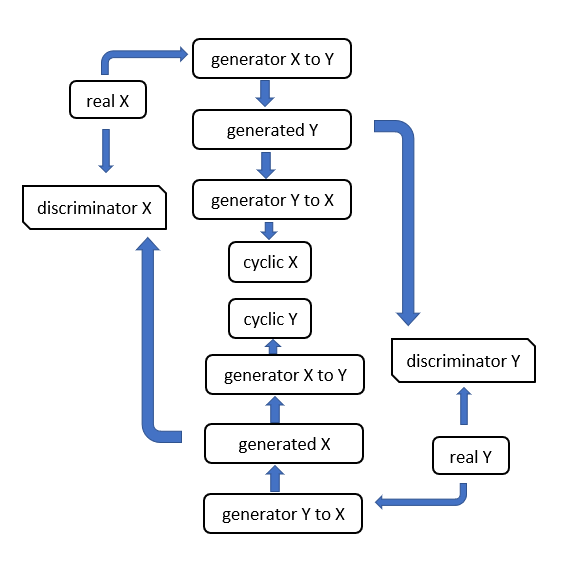
\includegraphics[width=0.5\textwidth]{./images/flux.png}
\hspace{1mm}
\label{flux}
\caption{simplified scheme of the architecture} 
\end{figure}

The model simplified representation is shown in figure~\ref{flux}. An image from the domain $X$ is fed to the generator that generates an image $Y$. This generated image $Y$ passed to the discriminator, which judged if it is real $(1)$ or fake-generated $(0)$. This same image generated $Y$ is the input of generator $Y$ to $X$, to convert it back to the original image $X$. The same process occurs for the $Y$ domain. Both discriminators receive two inputs: one generated and one real.      


\section{Results}
discuss our results only, Evaluation Metrics, Analysis of loss function, Limitations and Discussions


\section{Conclusion}



\bibliographystyle{abbrv}
\bibliography{bibliography}

% \clearpage
% \onecolumn
% \begin{appendices}

% \section{App} \label{sec:appendix-1}
 
% \newpage

% \end{appendices}
\end{document}